\documentclass{beamer}
\usetheme{metropolis}
\usepackage{graphicx}
\usepackage{subfig}
\usepackage{tcolorbox}
\title{Calculus-Based Physics-2: Electricity, Magnetism, and Thermodynamics (PHYS180-02): Unit 6}
\author{Jordan Hanson}
\institute{Whittier College Department of Physics and Astronomy}

\begin{document}
\maketitle

\section{Summary}

\begin{frame}{Summary}
\textbf{Reading: Chapter 16.1 - 16.3} \\ \vspace{0.5cm}
\textit{Resolving an issue with Amp\`{e}re's Law}
\begin{enumerate}
\item The Maxwell-Amp\`{e}re Law
\item Maxwell's Equations
\end{enumerate}
\textit{E-field $\rightarrow$ B-field $\rightarrow$ E-field $\rightarrow$ ...}
\begin{enumerate}
\item Electromagnetic wave equation
\item Energy density and radiation pressure
\end{enumerate}
\end{frame}

\section{Resolving an issue with  Amp\`{e}re's Law}

\begin{frame}{Resolving an issue with  Amp\`{e}re's Law}
\begin{figure}
\centering
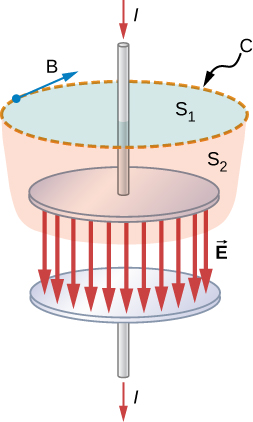
\includegraphics[width=0.35\textwidth]{figures/surface.jpeg}
\caption{\label{fig:surf} Two surfaces S1 and S2, for application of Amp\`{e}re's Law.}
\end{figure}
\end{frame}

\begin{frame}{Resolving an issue with  Amp\`{e}re's Law}
\begin{figure}
\centering
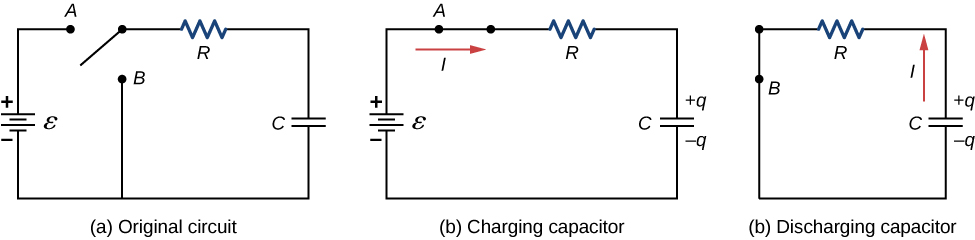
\includegraphics[width=0.75\textwidth]{figures/cap.jpeg}
\caption{\label{fig:surf2} Recall how we obtain the voltage of a charging capacitor.}
\end{figure}
\end{frame}

\begin{frame}{Resolving an issue with  Amp\`{e}re's Law}
The voltage of a charging capacitor in $RC$ circuit:
\begin{equation}
V_{\rm C} (t) = \epsilon \left( 1 - \exp(-t/\tau) \right)
\end{equation}
Let $\tau = RC$.  But what happens when we think more carefully about Fig. \ref{fig:surf}?
\begin{itemize}
\item Isn't I = 0 if you use surface 2 for Amp\`{e}re's Law?
\item What about the changing electric field?  Might there be a magnetic field? (Think of Faraday's law...)
\end{itemize}
\end{frame}

\begin{frame}{Resolving an issue with  Amp\`{e}re's Law}
Surface 1 versus surface 2: 
\begin{align}
\oint_{S1} \vec{B} \cdot d\vec{s} &= \mu_0 I_{in} \\
\oint_{S2} \vec{B} \cdot d\vec{s} &= 0
\end{align}
Maxwell added a \textit{displacement current:}
\begin{equation}
I_d = \epsilon_0 \frac{d\phi_E}{dt}
\end{equation}
so that
\begin{equation}
\oint \vec{B} \cdot d\vec{s} = \mu_0 (I + I_d)
\end{equation}
Both surfaces should now be equivalent (verify that $I(t) = I_d (t)$).
\end{frame}

\begin{frame}{Resolving an issue with  Amp\`{e}re's Law}
\begin{tcolorbox}[colback=white,colframe=black!100!black,title=The Maxwell-Amp\`{e}re Law]
\begin{equation}
\oint \vec{B} \cdot d\vec{s} = \mu_0 (I + I_d)
\end{equation}
\end{tcolorbox}
\begin{itemize}
\item Resolves displacement current issue
\item Relates integral of B-field to changing E-field
\end{itemize}
\end{frame}

\section{Maxwell's Equations - All of Electromagnetism}

\begin{frame}{Maxwell's Equations}
\begin{tcolorbox}[colback=white,colframe=black!100!black,title=Maxwell's Equations]
\begin{align}
\oint \vec{E} \cdot d\vec{A} &= \frac{Q_{in}}{\epsilon_0} \\
\oint \vec{B} \cdot d\vec{A} &= 0 \\
\oint \vec{E} \cdot d\vec{s} &= -\mu_0 \frac{d\phi_m}{dt} \\
\oint \vec{B} \cdot d\vec{s} &= \mu_0 I + \epsilon_o \mu_0 \frac{d\phi_E}{dt}
\end{align}
\end{tcolorbox}
Forces:
\begin{equation}
\vec{F} = q \vec{E} + q\vec{v} \times \vec{B}
\end{equation}
\end{frame}

\section{Electromagnetic Wave Equation}

\begin{frame}{Electromagnetic Wave Equation}
\begin{figure}
\centering
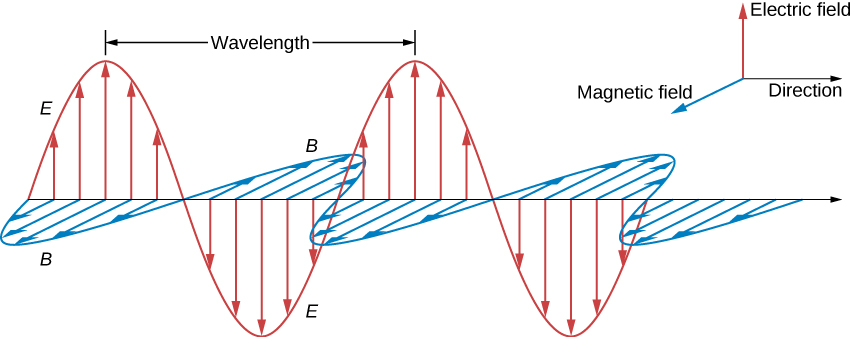
\includegraphics[width=0.5\textwidth]{figures/wave1.jpeg}
\caption{\label{fig:wave1} Consider a slice of volume with a 3D electric field \textit{propagating} in the x-direction.}
\end{figure}
\end{frame}

\begin{frame}{Electromagnetic Wave Equation}
\begin{enumerate}
\item Define box, and show that the flux from $E_y$ is zero
\item Same for $E_z$.
\item Net flux is from $E_x$, but $Q_{in} = 0$.  What does this imply?
\item Integrate $E_y$ around side 3, assuming $\Delta x$ is small
\item Consider side 3 magnetic flux... 
\end{enumerate}
\end{frame}

\begin{frame}{Electromagnetic Wave Equation}
\begin{figure}
\centering
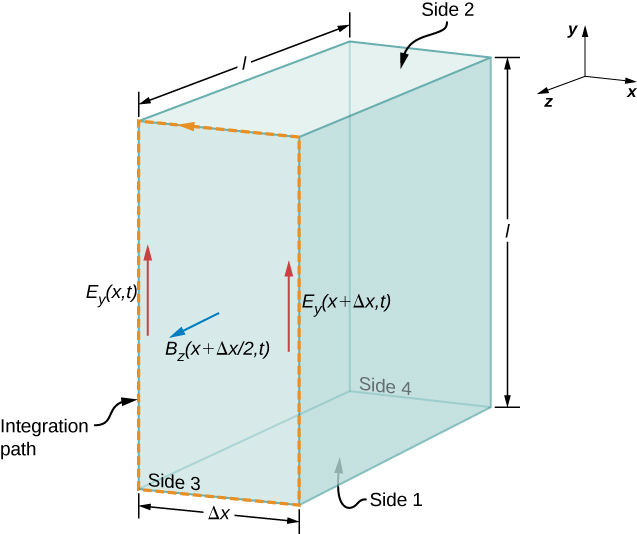
\includegraphics[width=0.55\textwidth]{figures/wave2.jpeg}
\caption{\label{fig:wave2} Consider a slice of volume with a 3D electric field \textit{propagating} in the x-direction.}
\end{figure}
\end{frame}

\begin{frame}{Electromagnetic Wave Equation}
\begin{enumerate}
\item Apply Faraday's law to side 3.
\item Repeat this combination for side 2.
\item Apply Maxwell-Amp\`{e}re's Law to sides 3 and 2.
\item Summarize four results.
\item Combine them to obtain \textbf{the wave equation.}
\item Solve wave equation...what is implied about $\epsilon_0$ and $\mu_0$?
\end{enumerate}
\end{frame}

\begin{frame}{Electromagnetic Wave Equation}
\begin{figure}
\centering
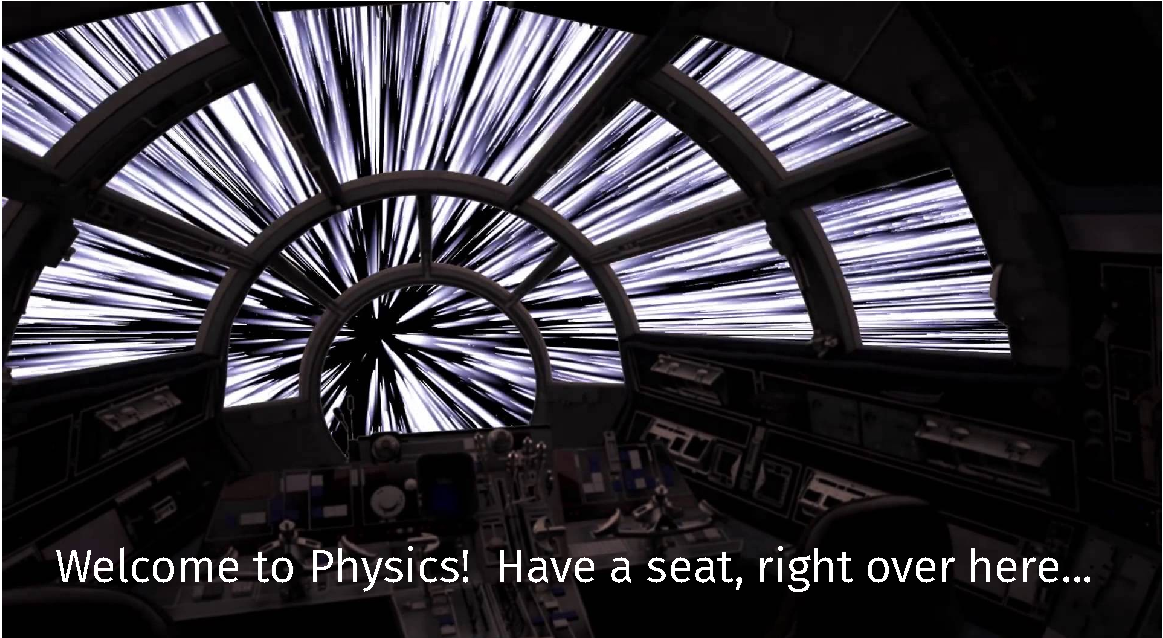
\includegraphics[width=0.85\textwidth]{figures/hyper.pdf}
\caption{\label{fig:hyper} Welcome to physics.}
\end{figure}
\end{frame}

\begin{frame}{Electromagnetic Wave Equation}
\begin{figure}
\centering

\includegraphics[width=0.85\textwidth]{figures/cat.jpeg}
\caption{\label{fig:cat} Welcome to physics.}
\end{figure}
\end{frame}

\section{Energy Density and Radiation Pressure}

\begin{frame}{Energy Density and Radiation Pressure}
Electromagnetic wave:
\begin{equation}
\vec{E}(x,t) = E_0 \cos(k(x-ct)) \hat{x}
\end{equation}
Let $\omega = ck$ so that
\begin{equation}
\vec{E}(x,t) = E_0 \cos(kx - \omega t) \hat{x}
\end{equation}
What is $k$? What does this \textit{propagator} function do?
\end{frame}

\begin{frame}{Energy Density and Radiation Pressure}
\begin{figure}
\centering
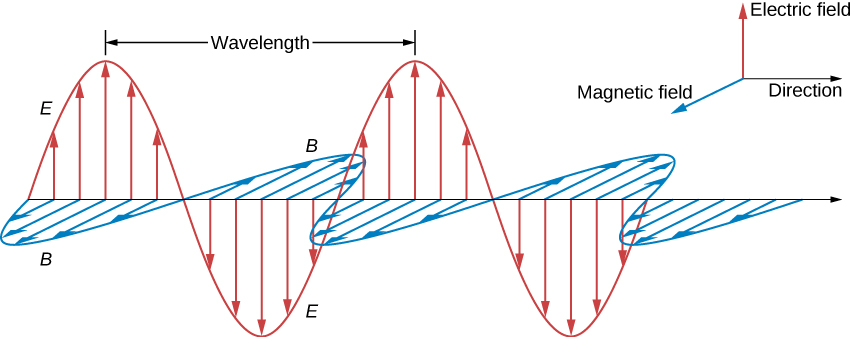
\includegraphics[width=0.7\textwidth]{figures/wave1.jpeg}
\caption{\label{fig:wave3} The E and B-fields of an electromagnetic wave.}
\end{figure}
\end{frame}

\begin{frame}{Energy Density and Radiation Pressure}
But haven't we shown that E and B-fields contain energy?  For capacitors:
\begin{equation}
U = \frac{1}{2}\frac{Q^2}{C}
\end{equation}
For inductors:
\begin{equation}
U = \frac{1}{2}LI^2
\end{equation}
\begin{itemize}
\item Re-derive each of these on the board.
\item Derive U for a \textit{parallel-plate capacitor}, and \textit{solenoid.}
\end{itemize}
\end{frame}

\begin{frame}{Energy Density and Radiation Pressure}
Use these to obtain U:
\begin{align}
C &= \frac{\epsilon_0 A}{d} \\
L &= \mu_0 n^2 V
\end{align}
\begin{itemize}
\item Obtain $u_E$ and $u_B$, the energy densities for each.
\item Get the total $u_{EM}$.
\end{itemize}
\end{frame}

\begin{frame}{Energy Density and Radiation Pressure}
The total energy density of an electromagnetic wave:
\begin{equation}
u_{EM} = \epsilon_0 E^2
\end{equation}
Radiation pressure: show that the units of the energy density are that of a \textit{pressure.}
\end{frame}

\begin{frame}{Energy Density and Radiation Pressure}
Radiation pressure: energy carried by electromagnetic waves can move objects...
\begin{align}
p &= I/c \\
p &= 2I/c
\end{align}
I is the intensity in Watts per meter squared, $c$ is the speed of light, and $p$ is the energy density or radiation pressure.  Example: sunlight intensity is 1370 Watts per meter squared in space.  What about a laser? \\ \vspace{0.5cm}
\alert{Examples.}
\end{frame}

\section{The Electromagnetic Spectrum}

\begin{frame}{Energy Density and Radiation Pressure}
\begin{figure}
\centering
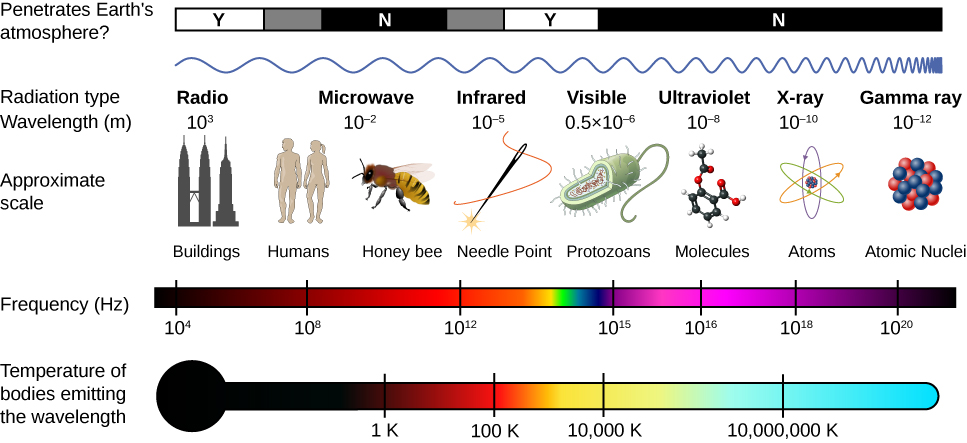
\includegraphics[width=0.8\textwidth]{figures/spectrum.jpeg}
\caption{\label{fig:spectrum} The electromagnetic spectrum.}
\end{figure}
\end{frame}

\begin{frame}{Summary}
\textbf{Reading: Chapter 16.1 - 16.3} \\ \vspace{0.5cm}
\textit{Resolving an issue with Amp\`{e}re's Law}
\begin{enumerate}
\item The Maxwell-Amp\`{e}re Law
\item Maxwell's Equations
\end{enumerate}
\textit{E-field $\rightarrow$ B-field $\rightarrow$ E-field $\rightarrow$ ...}
\begin{enumerate}
\item Electromagnetic wave equation
\item Energy density and radiation pressure
\end{enumerate}
\end{frame}

\end{document}
